\documentclass[1p]{elsarticle_modified}
%\bibliographystyle{elsarticle-num}

%\usepackage[colorlinks]{hyperref}
%\usepackage{abbrmath_seonhwa} %\Abb, \Ascr, \Acal ,\Abf, \Afrak
\usepackage{amsfonts}
\usepackage{amssymb}
\usepackage{amsmath}
\usepackage{amsthm}
\usepackage{scalefnt}
\usepackage{amsbsy}
\usepackage{kotex}
\usepackage{caption}
\usepackage{subfig}
\usepackage{color}
\usepackage{graphicx}
\usepackage{xcolor} %% white, black, red, green, blue, cyan, magenta, yellow
\usepackage{float}
\usepackage{setspace}
\usepackage{hyperref}

\usepackage{tikz}
\usetikzlibrary{arrows}

\usepackage{multirow}
\usepackage{array} % fixed length table
\usepackage{hhline}

%%%%%%%%%%%%%%%%%%%%%
\makeatletter
\renewcommand*\env@matrix[1][\arraystretch]{%
	\edef\arraystretch{#1}%
	\hskip -\arraycolsep
	\let\@ifnextchar\new@ifnextchar
	\array{*\c@MaxMatrixCols c}}
\makeatother %https://tex.stackexchange.com/questions/14071/how-can-i-increase-the-line-spacing-in-a-matrix
%%%%%%%%%%%%%%%

\usepackage[normalem]{ulem}

\newcommand{\msout}[1]{\ifmmode\text{\sout{\ensuremath{#1}}}\else\sout{#1}\fi}
%SOURCE: \msout is \stkout macro in https://tex.stackexchange.com/questions/20609/strikeout-in-math-mode

\newcommand{\cancel}[1]{
	\ifmmode
	{\color{red}\msout{#1}}
	\else
	{\color{red}\sout{#1}}
	\fi
}

\newcommand{\add}[1]{
	{\color{blue}\uwave{#1}}
}

\newcommand{\replace}[2]{
	\ifmmode
	{\color{red}\msout{#1}}{\color{blue}\uwave{#2}}
	\else
	{\color{red}\sout{#1}}{\color{blue}\uwave{#2}}
	\fi
}

\newcommand{\Sol}{\mathcal{S}} %segment
\newcommand{\D}{D} %diagram
\newcommand{\A}{\mathcal{A}} %arc


%%%%%%%%%%%%%%%%%%%%%%%%%%%%%5 test

\def\sl{\operatorname{\textup{SL}}(2,\Cbb)}
\def\psl{\operatorname{\textup{PSL}}(2,\Cbb)}
\def\quan{\mkern 1mu \triangleright \mkern 1mu}

\theoremstyle{definition}
\newtheorem{thm}{Theorem}[section]
\newtheorem{prop}[thm]{Proposition}
\newtheorem{lem}[thm]{Lemma}
\newtheorem{ques}[thm]{Question}
\newtheorem{cor}[thm]{Corollary}
\newtheorem{defn}[thm]{Definition}
\newtheorem{exam}[thm]{Example}
\newtheorem{rmk}[thm]{Remark}
\newtheorem{alg}[thm]{Algorithm}

\newcommand{\I}{\sqrt{-1}}
\begin{document}

%\begin{frontmatter}
%
%\title{Boundary parabolic representations of knots up to 8 crossings}
%
%%% Group authors per affiliation:
%\author{Yunhi Cho} 
%\address{Department of Mathematics, University of Seoul, Seoul, Korea}
%\ead{yhcho@uos.ac.kr}
%
%
%\author{Seonhwa Kim} %\fnref{s_kim}}
%\address{Center for Geometry and Physics, Institute for Basic Science, Pohang, 37673, Korea}
%\ead{ryeona17@ibs.re.kr}
%
%\author{Hyuk Kim}
%\address{Department of Mathematical Sciences, Seoul National University, Seoul 08826, Korea}
%\ead{hyukkim@snu.ac.kr}
%
%\author{Seokbeom Yoon}
%\address{Department of Mathematical Sciences, Seoul National University, Seoul, 08826,  Korea}
%\ead{sbyoon15@snu.ac.kr}
%
%\begin{abstract}
%We find all boundary parabolic representation of knots up to 8 crossings.
%
%\end{abstract}
%\begin{keyword}
%    \MSC[2010] 57M25 
%\end{keyword}
%
%\end{frontmatter}

%\linenumbers
%\tableofcontents
%
\newcommand\colored[1]{\textcolor{white}{\rule[-0.35ex]{0.8em}{1.4ex}}\kern-0.8em\color{red} #1}%
%\newcommand\colored[1]{\textcolor{white}{ #1}\kern-2.17ex	\textcolor{white}{ #1}\kern-1.81ex	\textcolor{white}{ #1}\kern-2.15ex\color{red}#1	}

{\Large $\underline{12n_{0800}~(K12n_{0800})}$}

\setlength{\tabcolsep}{10pt}
\renewcommand{\arraystretch}{1.6}
\vspace{1cm}\begin{tabular}{m{100pt}>{\centering\arraybackslash}m{274pt}}
\multirow{5}{120pt}{
	\centering
	\includegraphics[width=112pt]{../../../GIT/diagram.site/Diagrams/png/2889_12n_0800.png}\\
\ \ \ A knot diagram\footnotemark}&
\allowdisplaybreaks
\textbf{Linearized knot diagam} \\
\cline{2-2}
 &
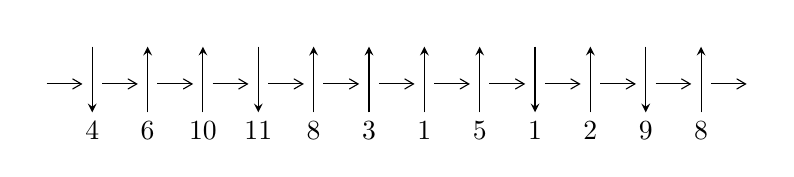
\begin{tikzpicture}[x=20pt, y=17pt]
	% nodes
	\node (C0) at (0, 0) {};
	\node (C1) at (1, 0) {};
	\node (C1U) at (1, +1) {};
	\node (C1D) at (1, -1) {4};

	\node (C2) at (2, 0) {};
	\node (C2U) at (2, +1) {};
	\node (C2D) at (2, -1) {6};

	\node (C3) at (3, 0) {};
	\node (C3U) at (3, +1) {};
	\node (C3D) at (3, -1) {10};

	\node (C4) at (4, 0) {};
	\node (C4U) at (4, +1) {};
	\node (C4D) at (4, -1) {11};

	\node (C5) at (5, 0) {};
	\node (C5U) at (5, +1) {};
	\node (C5D) at (5, -1) {8};

	\node (C6) at (6, 0) {};
	\node (C6U) at (6, +1) {};
	\node (C6D) at (6, -1) {3};

	\node (C7) at (7, 0) {};
	\node (C7U) at (7, +1) {};
	\node (C7D) at (7, -1) {1};

	\node (C8) at (8, 0) {};
	\node (C8U) at (8, +1) {};
	\node (C8D) at (8, -1) {5};

	\node (C9) at (9, 0) {};
	\node (C9U) at (9, +1) {};
	\node (C9D) at (9, -1) {1};

	\node (C10) at (10, 0) {};
	\node (C10U) at (10, +1) {};
	\node (C10D) at (10, -1) {2};

	\node (C11) at (11, 0) {};
	\node (C11U) at (11, +1) {};
	\node (C11D) at (11, -1) {9};

	\node (C12) at (12, 0) {};
	\node (C12U) at (12, +1) {};
	\node (C12D) at (12, -1) {8};
	\node (C13) at (13, 0) {};

	% arrows
	\draw[->,>={angle 60}]
	(C0) edge (C1) (C1) edge (C2) (C2) edge (C3) (C3) edge (C4) (C4) edge (C5) (C5) edge (C6) (C6) edge (C7) (C7) edge (C8) (C8) edge (C9) (C9) edge (C10) (C10) edge (C11) (C11) edge (C12) (C12) edge (C13) ;	\draw[->,>=stealth]
	(C1U) edge (C1D) (C2D) edge (C2U) (C3D) edge (C3U) (C4U) edge (C4D) (C5D) edge (C5U) (C6D) edge (C6U) (C7D) edge (C7U) (C8D) edge (C8U) (C9U) edge (C9D) (C10D) edge (C10U) (C11U) edge (C11D) (C12D) edge (C12U) ;
	\end{tikzpicture} \\
\hhline{~~} \\& 
\textbf{Solving Sequence} \\ \cline{2-2} 
 &
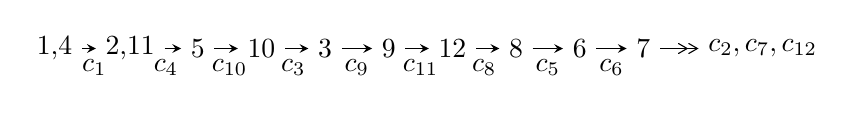
\begin{tikzpicture}[x=23pt, y=7pt]
	% node
	\node (A0) at (-1/8, 0) {1,4};
	\node (A1) at (17/16, 0) {2,11};
	\node (A2) at (17/8, 0) {5};
	\node (A3) at (25/8, 0) {10};
	\node (A4) at (33/8, 0) {3};
	\node (A5) at (41/8, 0) {9};
	\node (A6) at (49/8, 0) {12};
	\node (A7) at (57/8, 0) {8};
	\node (A8) at (65/8, 0) {6};
	\node (A9) at (73/8, 0) {7};
	\node (C1) at (1/2, -1) {$c_{1}$};
	\node (C2) at (13/8, -1) {$c_{4}$};
	\node (C3) at (21/8, -1) {$c_{10}$};
	\node (C4) at (29/8, -1) {$c_{3}$};
	\node (C5) at (37/8, -1) {$c_{9}$};
	\node (C6) at (45/8, -1) {$c_{11}$};
	\node (C7) at (53/8, -1) {$c_{8}$};
	\node (C8) at (61/8, -1) {$c_{5}$};
	\node (C9) at (69/8, -1) {$c_{6}$};
	\node (A10) at (11, 0) {$c_{2},c_{7},c_{12}$};

	% edge
	\draw[->,>=stealth]	
	(A0) edge (A1) (A1) edge (A2) (A2) edge (A3) (A3) edge (A4) (A4) edge (A5) (A5) edge (A6) (A6) edge (A7) (A7) edge (A8) (A8) edge (A9) ;
	\draw[->>,>={angle 60}]	
	(A9) edge (A10);
\end{tikzpicture} \\ 

\end{tabular} \\

\footnotetext{
The image of knot diagram is generated by the software ``\textbf{Draw programme}" developed by Andrew Bartholomew(\url{http://www.layer8.co.uk/maths/draw/index.htm\#Running-draw}), where we modified some parts for our purpose(\url{https://github.com/CATsTAILs/LinksPainter}).
}\phantom \\ \newline 
\centering \textbf{Ideals for irreducible components\footnotemark of $X_{\text{par}}$} 
 
\begin{align*}
I^u_{1}&=\langle 
-7.92227\times10^{321} u^{86}-3.69003\times10^{322} u^{85}+\cdots+2.21292\times10^{323} b-4.49196\times10^{322},\\
\phantom{I^u_{1}}&\phantom{= \langle  }-5.95683\times10^{322} u^{86}-2.93141\times10^{323} u^{85}+\cdots+2.21292\times10^{323} a-2.78972\times10^{323},\\
\phantom{I^u_{1}}&\phantom{= \langle  }u^{87}+5 u^{86}+\cdots+4 u+4\rangle \\
I^u_{2}&=\langle 
-3.25868\times10^{30} u^{29}+3.07384\times10^{31} u^{28}+\cdots+2.27509\times10^{31} b+1.25975\times10^{31},\\
\phantom{I^u_{2}}&\phantom{= \langle  }9.91315\times10^{31} u^{29}-7.89725\times10^{32} u^{28}+\cdots+2.27509\times10^{31} a+6.40206\times10^{32},\;u^{30}-8 u^{29}+\cdots+5 u+1\rangle \\
\\
\end{align*}
\raggedright * 2 irreducible components of $\dim_{\mathbb{C}}=0$, with total 117 representations.\\
\footnotetext{All coefficients of polynomials are rational numbers. But the coefficients are sometimes approximated in decimal forms when there is not enough margin.}
\newpage
\renewcommand{\arraystretch}{1}
\centering \section*{I. $I^u_{1}= \langle -7.92\times10^{321} u^{86}-3.69\times10^{322} u^{85}+\cdots+2.21\times10^{323} b-4.49\times10^{322},\;-5.96\times10^{322} u^{86}-2.93\times10^{323} u^{85}+\cdots+2.21\times10^{323} a-2.79\times10^{323},\;u^{87}+5 u^{86}+\cdots+4 u+4 \rangle$}
\flushleft \textbf{(i) Arc colorings}\\
\begin{tabular}{m{7pt} m{180pt} m{7pt} m{180pt} }
\flushright $a_{1}=$&$\begin{pmatrix}1\\0\end{pmatrix}$ \\
\flushright $a_{4}=$&$\begin{pmatrix}0\\u\end{pmatrix}$ \\
\flushright $a_{2}=$&$\begin{pmatrix}1\\u^2\end{pmatrix}$ \\
\flushright $a_{11}=$&$\begin{pmatrix}0.269184 u^{86}+1.32468 u^{85}+\cdots-19.4374 u+1.26065\\0.0358000 u^{86}+0.166749 u^{85}+\cdots-8.38995 u+0.202988\end{pmatrix}$ \\
\flushright $a_{5}=$&$\begin{pmatrix}-0.680199 u^{86}-3.41770 u^{85}+\cdots-15.4169 u-3.56450\\0.111567 u^{86}+0.524563 u^{85}+\cdots-0.0651331 u-1.20855\end{pmatrix}$ \\
\flushright $a_{10}=$&$\begin{pmatrix}0.222580 u^{86}+1.11462 u^{85}+\cdots-12.0392 u+1.14263\\0.0130509 u^{86}+0.0574080 u^{85}+\cdots-8.29540 u+0.111121\end{pmatrix}$ \\
\flushright $a_{3}=$&$\begin{pmatrix}-0.825564 u^{86}-4.14608 u^{85}+\cdots-9.76061 u-1.75430\\0.0999887 u^{86}+0.508035 u^{85}+\cdots+2.57177 u-0.461771\end{pmatrix}$ \\
\flushright $a_{9}=$&$\begin{pmatrix}0.235631 u^{86}+1.17203 u^{85}+\cdots-20.3346 u+1.25375\\0.0130509 u^{86}+0.0574080 u^{85}+\cdots-8.29540 u+0.111121\end{pmatrix}$ \\
\flushright $a_{12}=$&$\begin{pmatrix}0.395173 u^{86}+1.73507 u^{85}+\cdots-7.11517 u+0.677846\\-0.0892168 u^{86}-0.463239 u^{85}+\cdots-8.03508 u-0.827379\end{pmatrix}$ \\
\flushright $a_{8}=$&$\begin{pmatrix}0.323432 u^{86}+1.78313 u^{85}+\cdots-27.4861 u-4.51913\\0.0981978 u^{86}+0.425811 u^{85}+\cdots-5.99692 u+0.687737\end{pmatrix}$ \\
\flushright $a_{6}=$&$\begin{pmatrix}-0.356479 u^{86}-2.16611 u^{85}+\cdots+3.37461 u+3.34404\\-0.187301 u^{86}-0.872331 u^{85}+\cdots+0.697416 u-2.13808\end{pmatrix}$ \\
\flushright $a_{7}=$&$\begin{pmatrix}-0.225234 u^{86}-1.35732 u^{85}+\cdots+21.4892 u+5.20687\\-0.0981978 u^{86}-0.425811 u^{85}+\cdots+5.99692 u-0.687737\end{pmatrix}$\\&\end{tabular}
\flushleft \textbf{(ii) Obstruction class $= -1$}\\~\\
\flushleft \textbf{(iii) Cusp Shapes $= 0.150725 u^{86}+0.590384 u^{85}+\cdots-62.7762 u+6.33261$}\\~\\
\newpage\renewcommand{\arraystretch}{1}
\flushleft \textbf{(iv) u-Polynomials at the component}\newline \\
\begin{tabular}{m{50pt}|m{274pt}}
Crossings & \hspace{64pt}u-Polynomials at each crossing \\
\hline $$\begin{aligned}c_{1}\end{aligned}$$&$\begin{aligned}
&u^{87}-5 u^{86}+\cdots+4 u-4
\end{aligned}$\\
\hline $$\begin{aligned}c_{2},c_{6}\end{aligned}$$&$\begin{aligned}
&u^{87}+u^{86}+\cdots-352 u-43
\end{aligned}$\\
\hline $$\begin{aligned}c_{3}\end{aligned}$$&$\begin{aligned}
&u^{87}-10 u^{85}+\cdots-133313 u-18803
\end{aligned}$\\
\hline $$\begin{aligned}c_{4}\end{aligned}$$&$\begin{aligned}
&u^{87}-2 u^{86}+\cdots+6903 u-691
\end{aligned}$\\
\hline $$\begin{aligned}c_{5},c_{8}\end{aligned}$$&$\begin{aligned}
&u^{87}+4 u^{86}+\cdots-156 u-29
\end{aligned}$\\
\hline $$\begin{aligned}c_{7},c_{12}\end{aligned}$$&$\begin{aligned}
&u^{87}-40 u^{85}+\cdots+41988135 u-3861113
\end{aligned}$\\
\hline $$\begin{aligned}c_{9}\end{aligned}$$&$\begin{aligned}
&u^{87}-3 u^{86}+\cdots-1157278 u-318509
\end{aligned}$\\
\hline $$\begin{aligned}c_{10}\end{aligned}$$&$\begin{aligned}
&u^{87}-7 u^{86}+\cdots+884 u+71
\end{aligned}$\\
\hline $$\begin{aligned}c_{11}\end{aligned}$$&$\begin{aligned}
&u^{87}-2 u^{86}+\cdots+141578544 u+6358336
\end{aligned}$\\
\hline
\end{tabular}\\~\\
\newpage\renewcommand{\arraystretch}{1}
\flushleft \textbf{(v) Riley Polynomials at the component}\newline \\
\begin{tabular}{m{50pt}|m{274pt}}
Crossings & \hspace{64pt}Riley Polynomials at each crossing \\
\hline $$\begin{aligned}c_{1}\end{aligned}$$&$\begin{aligned}
&y^{87}-21 y^{86}+\cdots+632 y-16
\end{aligned}$\\
\hline $$\begin{aligned}c_{2},c_{6}\end{aligned}$$&$\begin{aligned}
&y^{87}-63 y^{86}+\cdots+52954 y-1849
\end{aligned}$\\
\hline $$\begin{aligned}c_{3}\end{aligned}$$&$\begin{aligned}
&y^{87}-20 y^{86}+\cdots+6084674411 y-353552809
\end{aligned}$\\
\hline $$\begin{aligned}c_{4}\end{aligned}$$&$\begin{aligned}
&y^{87}-36 y^{86}+\cdots+6991587 y-477481
\end{aligned}$\\
\hline $$\begin{aligned}c_{5},c_{8}\end{aligned}$$&$\begin{aligned}
&y^{87}+24 y^{86}+\cdots-20150 y-841
\end{aligned}$\\
\hline $$\begin{aligned}c_{7},c_{12}\end{aligned}$$&$\begin{aligned}
&y^{87}-80 y^{86}+\cdots-64642179821373 y-14908193598769
\end{aligned}$\\
\hline $$\begin{aligned}c_{9}\end{aligned}$$&$\begin{aligned}
&y^{87}+49 y^{86}+\cdots-124754575690068 y-101447983081
\end{aligned}$\\
\hline $$\begin{aligned}c_{10}\end{aligned}$$&$\begin{aligned}
&y^{87}- y^{86}+\cdots+1220520 y-5041
\end{aligned}$\\
\hline $$\begin{aligned}c_{11}\end{aligned}$$&$\begin{aligned}
&y^{87}+42 y^{86}+\cdots+15642609176560384 y-40428436688896
\end{aligned}$\\
\hline
\end{tabular}\\~\\
\newpage\flushleft \textbf{(vi) Complex Volumes and Cusp Shapes}
$$\begin{array}{c|c|c}  
\text{Solutions to }I^u_{1}& \I (\text{vol} + \sqrt{-1}CS) & \text{Cusp shape}\\
 \hline 
\begin{aligned}
u &= \phantom{-}0.912192 + 0.401975 I \\
a &= \phantom{-}1.71620 + 0.38603 I \\
b &= \phantom{-}1.218770 + 0.339427 I\end{aligned}
 & \phantom{-}2.78525 - 8.03445 I & \phantom{-0.000000 } 0 \\ \hline\begin{aligned}
u &= \phantom{-}0.912192 - 0.401975 I \\
a &= \phantom{-}1.71620 - 0.38603 I \\
b &= \phantom{-}1.218770 - 0.339427 I\end{aligned}
 & \phantom{-}2.78525 + 8.03445 I & \phantom{-0.000000 } 0 \\ \hline\begin{aligned}
u &= \phantom{-}0.063304 + 1.009710 I \\
a &= -0.384643 - 1.145980 I \\
b &= -0.348157 - 0.850557 I\end{aligned}
 & \phantom{-}5.78686 + 4.25193 I & \phantom{-0.000000 } 0 \\ \hline\begin{aligned}
u &= \phantom{-}0.063304 - 1.009710 I \\
a &= -0.384643 + 1.145980 I \\
b &= -0.348157 + 0.850557 I\end{aligned}
 & \phantom{-}5.78686 - 4.25193 I & \phantom{-0.000000 } 0 \\ \hline\begin{aligned}
u &= \phantom{-}0.453234 + 0.912797 I \\
a &= -0.028386 - 1.020130 I \\
b &= \phantom{-}0.41597 - 1.37970 I\end{aligned}
 & \phantom{-}5.44822 - 2.84020 I & \phantom{-0.000000 } 0 \\ \hline\begin{aligned}
u &= \phantom{-}0.453234 - 0.912797 I \\
a &= -0.028386 + 1.020130 I \\
b &= \phantom{-}0.41597 + 1.37970 I\end{aligned}
 & \phantom{-}5.44822 + 2.84020 I & \phantom{-0.000000 } 0 \\ \hline\begin{aligned}
u &= -0.694539 + 0.782085 I \\
a &= -0.64714 + 1.25869 I \\
b &= \phantom{-}0.410123 - 0.062150 I\end{aligned}
 & \phantom{-}9.43262 + 3.01438 I & \phantom{-0.000000 } 0 \\ \hline\begin{aligned}
u &= -0.694539 - 0.782085 I \\
a &= -0.64714 - 1.25869 I \\
b &= \phantom{-}0.410123 + 0.062150 I\end{aligned}
 & \phantom{-}9.43262 - 3.01438 I & \phantom{-0.000000 } 0 \\ \hline\begin{aligned}
u &= -0.416393 + 0.963809 I \\
a &= \phantom{-}0.339992 + 0.197096 I \\
b &= \phantom{-}0.467908 + 0.587539 I\end{aligned}
 & \phantom{-}3.48674 + 2.87950 I & \phantom{-0.000000 } 0 \\ \hline\begin{aligned}
u &= -0.416393 - 0.963809 I \\
a &= \phantom{-}0.339992 - 0.197096 I \\
b &= \phantom{-}0.467908 - 0.587539 I\end{aligned}
 & \phantom{-}3.48674 - 2.87950 I & \phantom{-0.000000 } 0\\
 \hline 
 \end{array}$$\newpage$$\begin{array}{c|c|c}  
\text{Solutions to }I^u_{1}& \I (\text{vol} + \sqrt{-1}CS) & \text{Cusp shape}\\
 \hline 
\begin{aligned}
u &= -0.785521 + 0.699014 I \\
a &= \phantom{-}0.993051 + 0.291711 I \\
b &= \phantom{-}1.49665 + 0.40739 I\end{aligned}
 & -3.25758 + 8.20249 I & \phantom{-0.000000 } 0 \\ \hline\begin{aligned}
u &= -0.785521 - 0.699014 I \\
a &= \phantom{-}0.993051 - 0.291711 I \\
b &= \phantom{-}1.49665 - 0.40739 I\end{aligned}
 & -3.25758 - 8.20249 I & \phantom{-0.000000 } 0 \\ \hline\begin{aligned}
u &= \phantom{-}0.816587 + 0.473890 I \\
a &= \phantom{-}1.81569 + 0.51492 I \\
b &= \phantom{-}0.719364 + 0.598319 I\end{aligned}
 & \phantom{-}3.76903 - 1.56318 I & \phantom{-}4.00000 + 3.26305 I \\ \hline\begin{aligned}
u &= \phantom{-}0.816587 - 0.473890 I \\
a &= \phantom{-}1.81569 - 0.51492 I \\
b &= \phantom{-}0.719364 - 0.598319 I\end{aligned}
 & \phantom{-}3.76903 + 1.56318 I & \phantom{-}4.00000 - 3.26305 I \\ \hline\begin{aligned}
u &= \phantom{-}0.147112 + 1.065990 I \\
a &= -0.401964 + 0.609701 I \\
b &= \phantom{-}0.111488 + 0.446761 I\end{aligned}
 & \phantom{-}2.45312 - 4.65946 I & \phantom{-0.000000 } 0 \\ \hline\begin{aligned}
u &= \phantom{-}0.147112 - 1.065990 I \\
a &= -0.401964 - 0.609701 I \\
b &= \phantom{-}0.111488 - 0.446761 I\end{aligned}
 & \phantom{-}2.45312 + 4.65946 I & \phantom{-0.000000 } 0 \\ \hline\begin{aligned}
u &= \phantom{-}0.931256 + 0.572305 I \\
a &= \phantom{-}0.785536 - 0.187780 I \\
b &= \phantom{-}1.57831 - 0.64495 I\end{aligned}
 & -3.96504 - 1.92363 I & \phantom{-0.000000 } 0 \\ \hline\begin{aligned}
u &= \phantom{-}0.931256 - 0.572305 I \\
a &= \phantom{-}0.785536 + 0.187780 I \\
b &= \phantom{-}1.57831 + 0.64495 I\end{aligned}
 & -3.96504 + 1.92363 I & \phantom{-0.000000 } 0 \\ \hline\begin{aligned}
u &= \phantom{-}0.892042 + 0.148083 I \\
a &= -0.422634 + 0.204443 I \\
b &= -0.593358 - 1.050630 I\end{aligned}
 & -2.69372 - 2.16255 I & -0.88908 + 4.42862 I \\ \hline\begin{aligned}
u &= \phantom{-}0.892042 - 0.148083 I \\
a &= -0.422634 - 0.204443 I \\
b &= -0.593358 + 1.050630 I\end{aligned}
 & -2.69372 + 2.16255 I & -0.88908 - 4.42862 I\\
 \hline 
 \end{array}$$\newpage$$\begin{array}{c|c|c}  
\text{Solutions to }I^u_{1}& \I (\text{vol} + \sqrt{-1}CS) & \text{Cusp shape}\\
 \hline 
\begin{aligned}
u &= -0.548120 + 0.988311 I \\
a &= \phantom{-}0.701455 - 0.520019 I \\
b &= -0.165990 - 0.329990 I\end{aligned}
 & \phantom{-}2.34699 - 1.37288 I & \phantom{-0.000000 } 0 \\ \hline\begin{aligned}
u &= -0.548120 - 0.988311 I \\
a &= \phantom{-}0.701455 + 0.520019 I \\
b &= -0.165990 + 0.329990 I\end{aligned}
 & \phantom{-}2.34699 + 1.37288 I & \phantom{-0.000000 } 0 \\ \hline\begin{aligned}
u &= -0.484874 + 1.021390 I \\
a &= \phantom{-}0.250420 - 0.050777 I \\
b &= \phantom{-}0.290233 + 0.553102 I\end{aligned}
 & \phantom{-}3.50028 + 2.86892 I & \phantom{-0.000000 } 0 \\ \hline\begin{aligned}
u &= -0.484874 - 1.021390 I \\
a &= \phantom{-}0.250420 + 0.050777 I \\
b &= \phantom{-}0.290233 - 0.553102 I\end{aligned}
 & \phantom{-}3.50028 - 2.86892 I & \phantom{-0.000000 } 0 \\ \hline\begin{aligned}
u &= \phantom{-}0.460721 + 0.683739 I \\
a &= \phantom{-}0.915361 + 0.110361 I \\
b &= \phantom{-}0.160669 - 0.135663 I\end{aligned}
 & \phantom{-}0.11406 - 1.55831 I & \phantom{-}1.29774 + 4.43942 I \\ \hline\begin{aligned}
u &= \phantom{-}0.460721 - 0.683739 I \\
a &= \phantom{-}0.915361 - 0.110361 I \\
b &= \phantom{-}0.160669 + 0.135663 I\end{aligned}
 & \phantom{-}0.11406 + 1.55831 I & \phantom{-}1.29774 - 4.43942 I \\ \hline\begin{aligned}
u &= -0.787268 + 0.887666 I \\
a &= -0.817774 + 1.041560 I \\
b &= \phantom{-}0.518701 + 0.366589 I\end{aligned}
 & \phantom{-}9.35877 + 9.75636 I & \phantom{-0.000000 } 0 \\ \hline\begin{aligned}
u &= -0.787268 - 0.887666 I \\
a &= -0.817774 - 1.041560 I \\
b &= \phantom{-}0.518701 - 0.366589 I\end{aligned}
 & \phantom{-}9.35877 - 9.75636 I & \phantom{-0.000000 } 0 \\ \hline\begin{aligned}
u &= -1.007710 + 0.645864 I \\
a &= -1.177580 - 0.334928 I \\
b &= -2.65128 + 0.45417 I\end{aligned}
 & -2.03670 + 4.04341 I & \phantom{-0.000000 } 0 \\ \hline\begin{aligned}
u &= -1.007710 - 0.645864 I \\
a &= -1.177580 + 0.334928 I \\
b &= -2.65128 - 0.45417 I\end{aligned}
 & -2.03670 - 4.04341 I & \phantom{-0.000000 } 0\\
 \hline 
 \end{array}$$\newpage$$\begin{array}{c|c|c}  
\text{Solutions to }I^u_{1}& \I (\text{vol} + \sqrt{-1}CS) & \text{Cusp shape}\\
 \hline 
\begin{aligned}
u &= \phantom{-}0.377151 + 1.147650 I \\
a &= -0.483019 - 0.604530 I \\
b &= \phantom{-}0.545999 + 0.569923 I\end{aligned}
 & \phantom{-}4.00465 + 2.11919 I & \phantom{-0.000000 } 0 \\ \hline\begin{aligned}
u &= \phantom{-}0.377151 - 1.147650 I \\
a &= -0.483019 + 0.604530 I \\
b &= \phantom{-}0.545999 - 0.569923 I\end{aligned}
 & \phantom{-}4.00465 - 2.11919 I & \phantom{-0.000000 } 0 \\ \hline\begin{aligned}
u &= -1.106240 + 0.490549 I \\
a &= -0.947435 - 0.589082 I \\
b &= -1.36762 + 0.53535 I\end{aligned}
 & -1.29962 + 1.65088 I & \phantom{-0.000000 } 0 \\ \hline\begin{aligned}
u &= -1.106240 - 0.490549 I \\
a &= -0.947435 + 0.589082 I \\
b &= -1.36762 - 0.53535 I\end{aligned}
 & -1.29962 - 1.65088 I & \phantom{-0.000000 } 0 \\ \hline\begin{aligned}
u &= -1.170960 + 0.382675 I \\
a &= \phantom{-}0.706683 - 0.206861 I \\
b &= \phantom{-}2.42929 - 1.12143 I\end{aligned}
 & \phantom{-}7.91042 + 1.84125 I & \phantom{-0.000000 } 0 \\ \hline\begin{aligned}
u &= -1.170960 - 0.382675 I \\
a &= \phantom{-}0.706683 + 0.206861 I \\
b &= \phantom{-}2.42929 + 1.12143 I\end{aligned}
 & \phantom{-}7.91042 - 1.84125 I & \phantom{-0.000000 } 0 \\ \hline\begin{aligned}
u &= \phantom{-}0.281224 + 0.709242 I \\
a &= -0.89796 + 1.43996 I \\
b &= -0.892007 - 0.507078 I\end{aligned}
 & -2.20998 - 5.06993 I & \phantom{-}1.66963 + 6.40826 I \\ \hline\begin{aligned}
u &= \phantom{-}0.281224 - 0.709242 I \\
a &= -0.89796 - 1.43996 I \\
b &= -0.892007 + 0.507078 I\end{aligned}
 & -2.20998 + 5.06993 I & \phantom{-}1.66963 - 6.40826 I \\ \hline\begin{aligned}
u &= -0.657198 + 0.307147 I \\
a &= \phantom{-}1.88727 + 0.07366 I \\
b &= \phantom{-}1.51953 - 0.47787 I\end{aligned}
 & -0.87663 + 6.37484 I & \phantom{-}6.19951 + 2.37879 I \\ \hline\begin{aligned}
u &= -0.657198 - 0.307147 I \\
a &= \phantom{-}1.88727 - 0.07366 I \\
b &= \phantom{-}1.51953 + 0.47787 I\end{aligned}
 & -0.87663 - 6.37484 I & \phantom{-}6.19951 - 2.37879 I\\
 \hline 
 \end{array}$$\newpage$$\begin{array}{c|c|c}  
\text{Solutions to }I^u_{1}& \I (\text{vol} + \sqrt{-1}CS) & \text{Cusp shape}\\
 \hline 
\begin{aligned}
u &= -1.155190 + 0.687197 I \\
a &= \phantom{-}0.719993 - 0.282618 I \\
b &= \phantom{-}1.68780 - 1.60413 I\end{aligned}
 & \phantom{-}8.22587 - 3.64595 I & \phantom{-0.000000 } 0 \\ \hline\begin{aligned}
u &= -1.155190 - 0.687197 I \\
a &= \phantom{-}0.719993 + 0.282618 I \\
b &= \phantom{-}1.68780 + 1.60413 I\end{aligned}
 & \phantom{-}8.22587 + 3.64595 I & \phantom{-0.000000 } 0 \\ \hline\begin{aligned}
u &= \phantom{-}0.643999 + 0.109479 I \\
a &= \phantom{-}1.061680 + 0.694693 I \\
b &= -0.030351 - 0.437816 I\end{aligned}
 & -3.39381 - 0.96598 I & \phantom{-}0.39517 + 7.21957 I \\ \hline\begin{aligned}
u &= \phantom{-}0.643999 - 0.109479 I \\
a &= \phantom{-}1.061680 - 0.694693 I \\
b &= -0.030351 + 0.437816 I\end{aligned}
 & -3.39381 + 0.96598 I & \phantom{-}0.39517 - 7.21957 I \\ \hline\begin{aligned}
u &= -0.566702 + 0.198795 I \\
a &= -1.98171 - 0.36620 I \\
b &= -1.39477 + 0.43507 I\end{aligned}
 & -2.60998 + 1.32687 I & \phantom{-}0.720881 - 0.280633 I \\ \hline\begin{aligned}
u &= -0.566702 - 0.198795 I \\
a &= -1.98171 + 0.36620 I \\
b &= -1.39477 - 0.43507 I\end{aligned}
 & -2.60998 - 1.32687 I & \phantom{-}0.720881 + 0.280633 I \\ \hline\begin{aligned}
u &= \phantom{-}0.741085 + 1.188570 I \\
a &= -0.341339 - 0.507587 I \\
b &= \phantom{-}0.647963 + 0.071670 I\end{aligned}
 & \phantom{-}3.72251 - 4.38135 I & \phantom{-0.000000 } 0 \\ \hline\begin{aligned}
u &= \phantom{-}0.741085 - 1.188570 I \\
a &= -0.341339 + 0.507587 I \\
b &= \phantom{-}0.647963 - 0.071670 I\end{aligned}
 & \phantom{-}3.72251 + 4.38135 I & \phantom{-0.000000 } 0 \\ \hline\begin{aligned}
u &= -0.572023 + 0.086882 I \\
a &= \phantom{-}1.75123 - 0.18932 I \\
b &= \phantom{-}0.202750 + 0.708885 I\end{aligned}
 & -3.14226 - 4.80021 I & \phantom{-}6.02675 + 3.57707 I \\ \hline\begin{aligned}
u &= -0.572023 - 0.086882 I \\
a &= \phantom{-}1.75123 + 0.18932 I \\
b &= \phantom{-}0.202750 - 0.708885 I\end{aligned}
 & -3.14226 + 4.80021 I & \phantom{-}6.02675 - 3.57707 I\\
 \hline 
 \end{array}$$\newpage$$\begin{array}{c|c|c}  
\text{Solutions to }I^u_{1}& \I (\text{vol} + \sqrt{-1}CS) & \text{Cusp shape}\\
 \hline 
\begin{aligned}
u &= -0.440749 + 0.367901 I \\
a &= \phantom{-}1.71358 + 0.03534 I \\
b &= \phantom{-}0.574482 - 0.388650 I\end{aligned}
 & \phantom{-}1.47462 - 0.14531 I & \phantom{-}7.13969 + 3.49282 I \\ \hline\begin{aligned}
u &= -0.440749 - 0.367901 I \\
a &= \phantom{-}1.71358 - 0.03534 I \\
b &= \phantom{-}0.574482 + 0.388650 I\end{aligned}
 & \phantom{-}1.47462 + 0.14531 I & \phantom{-}7.13969 - 3.49282 I \\ \hline\begin{aligned}
u &= -1.22331 + 0.82785 I \\
a &= -0.855548 + 0.140813 I \\
b &= -1.58797 + 1.11307 I\end{aligned}
 & \phantom{-}0.27819 + 8.09027 I & \phantom{-0.000000 } 0 \\ \hline\begin{aligned}
u &= -1.22331 - 0.82785 I \\
a &= -0.855548 - 0.140813 I \\
b &= -1.58797 - 1.11307 I\end{aligned}
 & \phantom{-}0.27819 - 8.09027 I & \phantom{-0.000000 } 0 \\ \hline\begin{aligned}
u &= -1.06015 + 1.03363 I \\
a &= \phantom{-}0.999482 + 0.206134 I \\
b &= \phantom{-}1.76783 - 0.88695 I\end{aligned}
 & \phantom{-}6.94845 + 10.55380 I & \phantom{-0.000000 } 0 \\ \hline\begin{aligned}
u &= -1.06015 - 1.03363 I \\
a &= \phantom{-}0.999482 - 0.206134 I \\
b &= \phantom{-}1.76783 + 0.88695 I\end{aligned}
 & \phantom{-}6.94845 - 10.55380 I & \phantom{-0.000000 } 0 \\ \hline\begin{aligned}
u &= \phantom{-}1.14479 + 1.03666 I \\
a &= \phantom{-}0.815763 - 0.109466 I \\
b &= \phantom{-}1.54275 + 1.18017 I\end{aligned}
 & \phantom{-}2.52234 - 3.55910 I & \phantom{-0.000000 } 0 \\ \hline\begin{aligned}
u &= \phantom{-}1.14479 - 1.03666 I \\
a &= \phantom{-}0.815763 + 0.109466 I \\
b &= \phantom{-}1.54275 - 1.18017 I\end{aligned}
 & \phantom{-}2.52234 + 3.55910 I & \phantom{-0.000000 } 0 \\ \hline\begin{aligned}
u &= -1.05813 + 1.12751 I \\
a &= \phantom{-}0.145464 + 0.730331 I \\
b &= \phantom{-}1.087400 - 0.008770 I\end{aligned}
 & \phantom{-}7.10114 - 2.70607 I & \phantom{-0.000000 } 0 \\ \hline\begin{aligned}
u &= -1.05813 - 1.12751 I \\
a &= \phantom{-}0.145464 - 0.730331 I \\
b &= \phantom{-}1.087400 + 0.008770 I\end{aligned}
 & \phantom{-}7.10114 + 2.70607 I & \phantom{-0.000000 } 0\\
 \hline 
 \end{array}$$\newpage$$\begin{array}{c|c|c}  
\text{Solutions to }I^u_{1}& \I (\text{vol} + \sqrt{-1}CS) & \text{Cusp shape}\\
 \hline 
\begin{aligned}
u &= -1.32042 + 0.82197 I \\
a &= -0.533477 - 0.058376 I \\
b &= -1.75928 + 0.27907 I\end{aligned}
 & \phantom{-}0.77190 + 4.16807 I & \phantom{-0.000000 } 0 \\ \hline\begin{aligned}
u &= -1.32042 - 0.82197 I \\
a &= -0.533477 + 0.058376 I \\
b &= -1.75928 - 0.27907 I\end{aligned}
 & \phantom{-}0.77190 - 4.16807 I & \phantom{-0.000000 } 0 \\ \hline\begin{aligned}
u &= -0.437998\phantom{ +0.000000I} \\
a &= \phantom{-}1.57305\phantom{ +0.000000I} \\
b &= \phantom{-}0.228308\phantom{ +0.000000I}\end{aligned}
 & \phantom{-}1.19704\phantom{ +0.000000I} & \phantom{-}7.87590\phantom{ +0.000000I} \\ \hline\begin{aligned}
u &= \phantom{-}1.24751 + 0.95031 I \\
a &= -0.736747 + 0.461163 I \\
b &= -2.02741 - 0.23872 I\end{aligned}
 & -6.47758 - 2.96918 I & \phantom{-0.000000 } 0 \\ \hline\begin{aligned}
u &= \phantom{-}1.24751 - 0.95031 I \\
a &= -0.736747 - 0.461163 I \\
b &= -2.02741 + 0.23872 I\end{aligned}
 & -6.47758 + 2.96918 I & \phantom{-0.000000 } 0 \\ \hline\begin{aligned}
u &= -1.18844 + 1.02512 I \\
a &= \phantom{-}1.004850 + 0.214529 I \\
b &= \phantom{-}2.19066 - 1.08284 I\end{aligned}
 & \phantom{-}5.7235 + 17.6063 I & \phantom{-0.000000 } 0 \\ \hline\begin{aligned}
u &= -1.18844 - 1.02512 I \\
a &= \phantom{-}1.004850 - 0.214529 I \\
b &= \phantom{-}2.19066 + 1.08284 I\end{aligned}
 & \phantom{-}5.7235 - 17.6063 I & \phantom{-0.000000 } 0 \\ \hline\begin{aligned}
u &= -1.09223 + 1.13307 I \\
a &= -0.662443 - 0.450886 I \\
b &= -2.15973 + 0.59397 I\end{aligned}
 & -0.10678 + 5.66380 I & \phantom{-0.000000 } 0 \\ \hline\begin{aligned}
u &= -1.09223 - 1.13307 I \\
a &= -0.662443 + 0.450886 I \\
b &= -2.15973 - 0.59397 I\end{aligned}
 & -0.10678 - 5.66380 I & \phantom{-0.000000 } 0 \\ \hline\begin{aligned}
u &= -0.112776 + 0.384345 I \\
a &= \phantom{-}5.57611 - 5.50713 I \\
b &= -1.006150 + 0.062796 I\end{aligned}
 & -0.0371163 - 0.0367021 I & -8.4334 - 13.9645 I\\
 \hline 
 \end{array}$$\newpage$$\begin{array}{c|c|c}  
\text{Solutions to }I^u_{1}& \I (\text{vol} + \sqrt{-1}CS) & \text{Cusp shape}\\
 \hline 
\begin{aligned}
u &= -0.112776 - 0.384345 I \\
a &= \phantom{-}5.57611 + 5.50713 I \\
b &= -1.006150 - 0.062796 I\end{aligned}
 & -0.0371163 + 0.0367021 I & -8.4334 + 13.9645 I \\ \hline\begin{aligned}
u &= \phantom{-}1.35698 + 0.93075 I \\
a &= \phantom{-}0.814355 - 0.101972 I \\
b &= \phantom{-}2.29464 + 1.25421 I\end{aligned}
 & \phantom{-}1.14531 - 9.78347 I & \phantom{-0.000000 } 0 \\ \hline\begin{aligned}
u &= \phantom{-}1.35698 - 0.93075 I \\
a &= \phantom{-}0.814355 + 0.101972 I \\
b &= \phantom{-}2.29464 - 1.25421 I\end{aligned}
 & \phantom{-}1.14531 + 9.78347 I & \phantom{-0.000000 } 0 \\ \hline\begin{aligned}
u &= -0.094411 + 0.338574 I \\
a &= \phantom{-}0.87849 - 1.44245 I \\
b &= \phantom{-}2.05669 + 0.94373 I\end{aligned}
 & \phantom{-}8.05058 + 0.40994 I & \phantom{-}18.7140 + 3.3872 I \\ \hline\begin{aligned}
u &= -0.094411 - 0.338574 I \\
a &= \phantom{-}0.87849 + 1.44245 I \\
b &= \phantom{-}2.05669 - 0.94373 I\end{aligned}
 & \phantom{-}8.05058 - 0.40994 I & \phantom{-}18.7140 - 3.3872 I \\ \hline\begin{aligned}
u &= \phantom{-}0.312702 + 0.159104 I \\
a &= \phantom{-}2.77994 - 0.20053 I \\
b &= \phantom{-}2.32458 + 2.43420 I\end{aligned}
 & \phantom{-}5.59090 - 6.35630 I & -0.1485 + 15.1289 I \\ \hline\begin{aligned}
u &= \phantom{-}0.312702 - 0.159104 I \\
a &= \phantom{-}2.77994 + 0.20053 I \\
b &= \phantom{-}2.32458 - 2.43420 I\end{aligned}
 & \phantom{-}5.59090 + 6.35630 I & -0.1485 - 15.1289 I \\ \hline\begin{aligned}
u &= -0.95311 + 1.37768 I \\
a &= \phantom{-}0.053807 + 0.760361 I \\
b &= \phantom{-}1.327890 - 0.448270 I\end{aligned}
 & \phantom{-}6.72564 - 9.19457 I & \phantom{-0.000000 } 0 \\ \hline\begin{aligned}
u &= -0.95311 - 1.37768 I \\
a &= \phantom{-}0.053807 - 0.760361 I \\
b &= \phantom{-}1.327890 + 0.448270 I\end{aligned}
 & \phantom{-}6.72564 + 9.19457 I & \phantom{-0.000000 } 0 \\ \hline\begin{aligned}
u &= \phantom{-}1.18578 + 1.18641 I \\
a &= -0.730372 + 0.476175 I \\
b &= -1.79404 - 0.86269 I\end{aligned}
 & -5.77689 - 5.71907 I & \phantom{-0.000000 } 0\\
 \hline 
 \end{array}$$\newpage$$\begin{array}{c|c|c}  
\text{Solutions to }I^u_{1}& \I (\text{vol} + \sqrt{-1}CS) & \text{Cusp shape}\\
 \hline 
\begin{aligned}
u &= \phantom{-}1.18578 - 1.18641 I \\
a &= -0.730372 - 0.476175 I \\
b &= -1.79404 + 0.86269 I\end{aligned}
 & -5.77689 + 5.71907 I & \phantom{-0.000000 } 0 \\ \hline\begin{aligned}
u &= \phantom{-}0.233582 + 0.040081 I \\
a &= -6.96917 - 1.14129 I \\
b &= -0.838345 + 0.317215 I\end{aligned}
 & \phantom{-}0.311077 - 0.458631 I & \phantom{-}2.75665 + 5.13065 I \\ \hline\begin{aligned}
u &= \phantom{-}0.233582 - 0.040081 I \\
a &= -6.96917 + 1.14129 I \\
b &= -0.838345 - 0.317215 I\end{aligned}
 & \phantom{-}0.311077 + 0.458631 I & \phantom{-}2.75665 - 5.13065 I \\ \hline\begin{aligned}
u &= \phantom{-}1.92037 + 0.28539 I \\
a &= -0.599470 + 0.151895 I \\
b &= -3.00149 - 0.04689 I\end{aligned}
 & -7.66564 - 0.71189 I & \phantom{-0.000000 } 0 \\ \hline\begin{aligned}
u &= \phantom{-}1.92037 - 0.28539 I \\
a &= -0.599470 - 0.151895 I \\
b &= -3.00149 + 0.04689 I\end{aligned}
 & -7.66564 + 0.71189 I & \phantom{-0.000000 } 0 \\ \hline\begin{aligned}
u &= \phantom{-}2.09382 + 0.09189 I \\
a &= -0.344115 - 0.080336 I \\
b &= -2.08465 - 0.48560 I\end{aligned}
 & -5.77352 - 2.12518 I & \phantom{-0.000000 } 0 \\ \hline\begin{aligned}
u &= \phantom{-}2.09382 - 0.09189 I \\
a &= -0.344115 + 0.080336 I \\
b &= -2.08465 + 0.48560 I\end{aligned}
 & -5.77352 + 2.12518 I & \phantom{-0.000000 } 0\\
 \hline 
 \end{array}$$\newpage\newpage\renewcommand{\arraystretch}{1}
\centering \section*{II. $I^u_{2}= \langle -3.26\times10^{30} u^{29}+3.07\times10^{31} u^{28}+\cdots+2.28\times10^{31} b+1.26\times10^{31},\;9.91\times10^{31} u^{29}-7.90\times10^{32} u^{28}+\cdots+2.28\times10^{31} a+6.40\times10^{32},\;u^{30}-8 u^{29}+\cdots+5 u+1 \rangle$}
\flushleft \textbf{(i) Arc colorings}\\
\begin{tabular}{m{7pt} m{180pt} m{7pt} m{180pt} }
\flushright $a_{1}=$&$\begin{pmatrix}1\\0\end{pmatrix}$ \\
\flushright $a_{4}=$&$\begin{pmatrix}0\\u\end{pmatrix}$ \\
\flushright $a_{2}=$&$\begin{pmatrix}1\\u^2\end{pmatrix}$ \\
\flushright $a_{11}=$&$\begin{pmatrix}-4.35726 u^{29}+34.7118 u^{28}+\cdots-11.4934 u-28.1398\\0.143233 u^{29}-1.35109 u^{28}+\cdots+2.21771 u-0.553715\end{pmatrix}$ \\
\flushright $a_{5}=$&$\begin{pmatrix}32.4699 u^{29}-264.608 u^{28}+\cdots+107.589 u+152.261\\1.04679 u^{29}-8.54165 u^{28}+\cdots+1.93436 u+6.39287\end{pmatrix}$ \\
\flushright $a_{10}=$&$\begin{pmatrix}-3.45609 u^{29}+26.9760 u^{28}+\cdots-8.62249 u-27.4399\\0.637967 u^{29}-5.66845 u^{28}+\cdots+3.94896 u-0.0272306\end{pmatrix}$ \\
\flushright $a_{3}=$&$\begin{pmatrix}29.2569 u^{29}-235.969 u^{28}+\cdots+90.1819 u+149.419\\-1.19067 u^{29}+11.3015 u^{28}+\cdots-10.4421 u+3.21100\end{pmatrix}$ \\
\flushright $a_{9}=$&$\begin{pmatrix}-2.81812 u^{29}+21.3075 u^{28}+\cdots-4.67353 u-27.4671\\0.637967 u^{29}-5.66845 u^{28}+\cdots+3.94896 u-0.0272306\end{pmatrix}$ \\
\flushright $a_{12}=$&$\begin{pmatrix}2.38336 u^{29}-20.9011 u^{28}+\cdots+12.2620 u+4.97176\\1.70365 u^{29}-14.7732 u^{28}+\cdots+7.33375 u+2.02151\end{pmatrix}$ \\
\flushright $a_{8}=$&$\begin{pmatrix}-5.57532 u^{29}+48.4654 u^{28}+\cdots-32.7344 u-13.3998\\0.313551 u^{29}-2.67450 u^{28}+\cdots+2.41495 u+0.394386\end{pmatrix}$ \\
\flushright $a_{6}=$&$\begin{pmatrix}36.6261 u^{29}-301.275 u^{28}+\cdots+128.389 u+157.033\\1.01379 u^{29}-8.31609 u^{28}+\cdots+2.17156 u+6.40119\end{pmatrix}$ \\
\flushright $a_{7}=$&$\begin{pmatrix}-5.88887 u^{29}+51.1399 u^{28}+\cdots-35.1493 u-13.7942\\0.313551 u^{29}-2.67450 u^{28}+\cdots+2.41495 u+0.394386\end{pmatrix}$\\&\end{tabular}
\flushleft \textbf{(ii) Obstruction class $= 1$}\\~\\
\flushleft \textbf{(iii) Cusp Shapes $= -73.4402 u^{29}+601.455 u^{28}+\cdots-270.631 u-331.472$}\\~\\
\newpage\renewcommand{\arraystretch}{1}
\flushleft \textbf{(iv) u-Polynomials at the component}\newline \\
\begin{tabular}{m{50pt}|m{274pt}}
Crossings & \hspace{64pt}u-Polynomials at each crossing \\
\hline $$\begin{aligned}c_{1}\end{aligned}$$&$\begin{aligned}
&u^{30}-8 u^{29}+\cdots+5 u+1
\end{aligned}$\\
\hline $$\begin{aligned}c_{2}\end{aligned}$$&$\begin{aligned}
&u^{30}-2 u^{29}+\cdots- u+1
\end{aligned}$\\
\hline $$\begin{aligned}c_{3}\end{aligned}$$&$\begin{aligned}
&u^{30}+7 u^{29}+\cdots-2 u+1
\end{aligned}$\\
\hline $$\begin{aligned}c_{4}\end{aligned}$$&$\begin{aligned}
&u^{30}+7 u^{29}+\cdots-4 u+17
\end{aligned}$\\
\hline $$\begin{aligned}c_{5}\end{aligned}$$&$\begin{aligned}
&u^{30}+7 u^{29}+\cdots+11 u+1
\end{aligned}$\\
\hline $$\begin{aligned}c_{6}\end{aligned}$$&$\begin{aligned}
&u^{30}+2 u^{29}+\cdots+u+1
\end{aligned}$\\
\hline $$\begin{aligned}c_{7}\end{aligned}$$&$\begin{aligned}
&u^{30}- u^{29}+\cdots-22 u+1
\end{aligned}$\\
\hline $$\begin{aligned}c_{8}\end{aligned}$$&$\begin{aligned}
&u^{30}-7 u^{29}+\cdots-11 u+1
\end{aligned}$\\
\hline $$\begin{aligned}c_{9}\end{aligned}$$&$\begin{aligned}
&u^{30}+6 u^{29}+\cdots+3 u+1
\end{aligned}$\\
\hline $$\begin{aligned}c_{10}\end{aligned}$$&$\begin{aligned}
&u^{30}+4 u^{28}+\cdots+9 u+1
\end{aligned}$\\
\hline $$\begin{aligned}c_{11}\end{aligned}$$&$\begin{aligned}
&u^{30}+5 u^{29}+\cdots+702 u+324
\end{aligned}$\\
\hline $$\begin{aligned}c_{12}\end{aligned}$$&$\begin{aligned}
&u^{30}+u^{29}+\cdots+22 u+1
\end{aligned}$\\
\hline
\end{tabular}\\~\\
\newpage\renewcommand{\arraystretch}{1}
\flushleft \textbf{(v) Riley Polynomials at the component}\newline \\
\begin{tabular}{m{50pt}|m{274pt}}
Crossings & \hspace{64pt}Riley Polynomials at each crossing \\
\hline $$\begin{aligned}c_{1}\end{aligned}$$&$\begin{aligned}
&y^{30}-16 y^{29}+\cdots-27 y+1
\end{aligned}$\\
\hline $$\begin{aligned}c_{2},c_{6}\end{aligned}$$&$\begin{aligned}
&y^{30}-14 y^{29}+\cdots-13 y+1
\end{aligned}$\\
\hline $$\begin{aligned}c_{3}\end{aligned}$$&$\begin{aligned}
&y^{30}-27 y^{29}+\cdots-10 y+1
\end{aligned}$\\
\hline $$\begin{aligned}c_{4}\end{aligned}$$&$\begin{aligned}
&y^{30}-51 y^{29}+\cdots-5762 y+289
\end{aligned}$\\
\hline $$\begin{aligned}c_{5},c_{8}\end{aligned}$$&$\begin{aligned}
&y^{30}+13 y^{29}+\cdots-17 y+1
\end{aligned}$\\
\hline $$\begin{aligned}c_{7},c_{12}\end{aligned}$$&$\begin{aligned}
&y^{30}+y^{29}+\cdots-162 y+1
\end{aligned}$\\
\hline $$\begin{aligned}c_{9}\end{aligned}$$&$\begin{aligned}
&y^{30}+10 y^{29}+\cdots+221 y+1
\end{aligned}$\\
\hline $$\begin{aligned}c_{10}\end{aligned}$$&$\begin{aligned}
&y^{30}+8 y^{29}+\cdots-103 y+1
\end{aligned}$\\
\hline $$\begin{aligned}c_{11}\end{aligned}$$&$\begin{aligned}
&y^{30}+7 y^{29}+\cdots+1799172 y+104976
\end{aligned}$\\
\hline
\end{tabular}\\~\\
\newpage\flushleft \textbf{(vi) Complex Volumes and Cusp Shapes}
$$\begin{array}{c|c|c}  
\text{Solutions to }I^u_{2}& \I (\text{vol} + \sqrt{-1}CS) & \text{Cusp shape}\\
 \hline 
\begin{aligned}
u &= -0.922928 + 0.587538 I \\
a &= -0.945123 - 0.371366 I \\
b &= -2.12791 - 0.57187 I\end{aligned}
 & -3.96611 + 7.21759 I & -0.87488 - 5.62385 I \\ \hline\begin{aligned}
u &= -0.922928 - 0.587538 I \\
a &= -0.945123 + 0.371366 I \\
b &= -2.12791 + 0.57187 I\end{aligned}
 & -3.96611 - 7.21759 I & -0.87488 + 5.62385 I \\ \hline\begin{aligned}
u &= \phantom{-}0.704491 + 0.496236 I \\
a &= \phantom{-}1.57500 - 0.31600 I \\
b &= \phantom{-}1.46524 + 0.51141 I\end{aligned}
 & -1.00133 - 6.83745 I & \phantom{-}2.05753 + 13.48275 I \\ \hline\begin{aligned}
u &= \phantom{-}0.704491 - 0.496236 I \\
a &= \phantom{-}1.57500 + 0.31600 I \\
b &= \phantom{-}1.46524 - 0.51141 I\end{aligned}
 & -1.00133 + 6.83745 I & \phantom{-}2.05753 - 13.48275 I \\ \hline\begin{aligned}
u &= \phantom{-}0.386560 + 1.109940 I \\
a &= -0.051401 - 0.462394 I \\
b &= \phantom{-}0.304135 - 0.577341 I\end{aligned}
 & \phantom{-}2.50276 - 3.64171 I & \phantom{-}2.92014 + 2.19640 I \\ \hline\begin{aligned}
u &= \phantom{-}0.386560 - 1.109940 I \\
a &= -0.051401 + 0.462394 I \\
b &= \phantom{-}0.304135 + 0.577341 I\end{aligned}
 & \phantom{-}2.50276 + 3.64171 I & \phantom{-}2.92014 - 2.19640 I \\ \hline\begin{aligned}
u &= -0.263153 + 1.160860 I \\
a &= -0.431578 - 0.621044 I \\
b &= -0.407030 - 0.132485 I\end{aligned}
 & \phantom{-}2.87178 + 3.78144 I & \phantom{-}6.31019 - 4.19604 I \\ \hline\begin{aligned}
u &= -0.263153 - 1.160860 I \\
a &= -0.431578 + 0.621044 I \\
b &= -0.407030 + 0.132485 I\end{aligned}
 & \phantom{-}2.87178 - 3.78144 I & \phantom{-}6.31019 + 4.19604 I \\ \hline\begin{aligned}
u &= \phantom{-}0.500940 + 0.629952 I \\
a &= \phantom{-}1.68166 - 0.06066 I \\
b &= \phantom{-}0.303310 + 0.498258 I\end{aligned}
 & \phantom{-}1.43876 - 0.76884 I & \phantom{-}6.64471 + 4.27009 I \\ \hline\begin{aligned}
u &= \phantom{-}0.500940 - 0.629952 I \\
a &= \phantom{-}1.68166 + 0.06066 I \\
b &= \phantom{-}0.303310 - 0.498258 I\end{aligned}
 & \phantom{-}1.43876 + 0.76884 I & \phantom{-}6.64471 - 4.27009 I\\
 \hline 
 \end{array}$$\newpage$$\begin{array}{c|c|c}  
\text{Solutions to }I^u_{2}& \I (\text{vol} + \sqrt{-1}CS) & \text{Cusp shape}\\
 \hline 
\begin{aligned}
u &= -0.743487 + 0.011194 I \\
a &= -1.58893 + 0.46371 I \\
b &= -0.672210 - 0.441056 I\end{aligned}
 & -3.76793 - 4.74109 I & -6.96064 + 3.57575 I \\ \hline\begin{aligned}
u &= -0.743487 - 0.011194 I \\
a &= -1.58893 - 0.46371 I \\
b &= -0.672210 + 0.441056 I\end{aligned}
 & -3.76793 + 4.74109 I & -6.96064 - 3.57575 I \\ \hline\begin{aligned}
u &= \phantom{-}0.641333 + 0.136681 I \\
a &= -0.906364 + 1.074960 I \\
b &= -0.329411 - 0.850433 I\end{aligned}
 & -3.51250 + 0.24334 I & -1.82124 + 2.49290 I \\ \hline\begin{aligned}
u &= \phantom{-}0.641333 - 0.136681 I \\
a &= -0.906364 - 1.074960 I \\
b &= -0.329411 + 0.850433 I\end{aligned}
 & -3.51250 - 0.24334 I & -1.82124 - 2.49290 I \\ \hline\begin{aligned}
u &= -0.609580 + 0.204219 I \\
a &= \phantom{-}0.407913 + 0.650635 I \\
b &= \phantom{-}2.23585 + 0.71430 I\end{aligned}
 & \phantom{-}7.62000 + 0.50528 I & \phantom{-}0.258078 - 0.196315 I \\ \hline\begin{aligned}
u &= -0.609580 - 0.204219 I \\
a &= \phantom{-}0.407913 - 0.650635 I \\
b &= \phantom{-}2.23585 - 0.71430 I\end{aligned}
 & \phantom{-}7.62000 - 0.50528 I & \phantom{-}0.258078 + 0.196315 I \\ \hline\begin{aligned}
u &= -0.573695\phantom{ +0.000000I} \\
a &= -3.33723\phantom{ +0.000000I} \\
b &= -0.970491\phantom{ +0.000000I}\end{aligned}
 & -0.112514\phantom{ +0.000000I} & -7.33930\phantom{ +0.000000I} \\ \hline\begin{aligned}
u &= -0.234236 + 0.490295 I \\
a &= -0.02926 + 1.74200 I \\
b &= \phantom{-}1.79609 + 1.69689 I\end{aligned}
 & \phantom{-}5.83320 - 6.00958 I & \phantom{-}10.35590 + 0.19003 I \\ \hline\begin{aligned}
u &= -0.234236 - 0.490295 I \\
a &= -0.02926 - 1.74200 I \\
b &= \phantom{-}1.79609 - 1.69689 I\end{aligned}
 & \phantom{-}5.83320 + 6.00958 I & \phantom{-}10.35590 - 0.19003 I \\ \hline\begin{aligned}
u &= \phantom{-}1.17894 + 0.89891 I \\
a &= -0.806852 + 0.440198 I \\
b &= -1.97344 - 0.14521 I\end{aligned}
 & -6.51184 - 2.43468 I & \phantom{-0.000000 } 0\\
 \hline 
 \end{array}$$\newpage$$\begin{array}{c|c|c}  
\text{Solutions to }I^u_{2}& \I (\text{vol} + \sqrt{-1}CS) & \text{Cusp shape}\\
 \hline 
\begin{aligned}
u &= \phantom{-}1.17894 - 0.89891 I \\
a &= -0.806852 - 0.440198 I \\
b &= -1.97344 + 0.14521 I\end{aligned}
 & -6.51184 + 2.43468 I & \phantom{-0.000000 } 0 \\ \hline\begin{aligned}
u &= -1.24538 + 0.97708 I \\
a &= -0.714351 - 0.298346 I \\
b &= -2.34521 + 0.62696 I\end{aligned}
 & -0.25045 + 5.04299 I & \phantom{-0.000000 } 0 \\ \hline\begin{aligned}
u &= -1.24538 - 0.97708 I \\
a &= -0.714351 + 0.298346 I \\
b &= -2.34521 - 0.62696 I\end{aligned}
 & -0.25045 - 5.04299 I & \phantom{-0.000000 } 0 \\ \hline\begin{aligned}
u &= \phantom{-}1.15151 + 1.21077 I \\
a &= -0.710752 + 0.517304 I \\
b &= -1.70800 - 0.84973 I\end{aligned}
 & -5.59793 - 5.98728 I & \phantom{-0.000000 } 0 \\ \hline\begin{aligned}
u &= \phantom{-}1.15151 - 1.21077 I \\
a &= -0.710752 - 0.517304 I \\
b &= -1.70800 + 0.84973 I\end{aligned}
 & -5.59793 + 5.98728 I & \phantom{-0.000000 } 0 \\ \hline\begin{aligned}
u &= -0.245930\phantom{ +0.000000I} \\
a &= -19.5202\phantom{ +0.000000I} \\
b &= -1.01937\phantom{ +0.000000I}\end{aligned}
 & \phantom{-}0.0131283\phantom{ +0.000000I} & -196.150\phantom{ +0.000000I} \\ \hline\begin{aligned}
u &= \phantom{-}1.88508 + 0.17326 I \\
a &= -0.620542 + 0.087183 I \\
b &= -3.08908 + 0.19184 I\end{aligned}
 & -7.58112 - 1.13122 I & \phantom{-0.000000 } 0 \\ \hline\begin{aligned}
u &= \phantom{-}1.88508 - 0.17326 I \\
a &= -0.620542 - 0.087183 I \\
b &= -3.08908 - 0.19184 I\end{aligned}
 & -7.58112 + 1.13122 I & \phantom{-0.000000 } 0 \\ \hline\begin{aligned}
u &= \phantom{-}1.97973 + 0.12368 I \\
a &= -0.430688 - 0.048129 I \\
b &= -1.95742 - 0.56422 I\end{aligned}
 & -6.12186 - 2.02764 I & \phantom{-0.000000 } 0 \\ \hline\begin{aligned}
u &= \phantom{-}1.97973 - 0.12368 I \\
a &= -0.430688 + 0.048129 I \\
b &= -1.95742 + 0.56422 I\end{aligned}
 & -6.12186 + 2.02764 I & \phantom{-0.000000 } 0\\
 \hline 
 \end{array}$$\newpage
\newpage\renewcommand{\arraystretch}{1}
\centering \section*{ III. u-Polynomials}
\begin{tabular}{m{50pt}|m{274pt}}
Crossings & \hspace{64pt}u-Polynomials at each crossing \\
\hline $$\begin{aligned}c_{1}\end{aligned}$$&$\begin{aligned}
&(u^{30}-8 u^{29}+\cdots+5 u+1)(u^{87}-5 u^{86}+\cdots+4 u-4)
\end{aligned}$\\
\hline $$\begin{aligned}c_{2}\end{aligned}$$&$\begin{aligned}
&(u^{30}-2 u^{29}+\cdots- u+1)(u^{87}+u^{86}+\cdots-352 u-43)
\end{aligned}$\\
\hline $$\begin{aligned}c_{3}\end{aligned}$$&$\begin{aligned}
&(u^{30}+7 u^{29}+\cdots-2 u+1)(u^{87}-10 u^{85}+\cdots-133313 u-18803)
\end{aligned}$\\
\hline $$\begin{aligned}c_{4}\end{aligned}$$&$\begin{aligned}
&(u^{30}+7 u^{29}+\cdots-4 u+17)(u^{87}-2 u^{86}+\cdots+6903 u-691)
\end{aligned}$\\
\hline $$\begin{aligned}c_{5}\end{aligned}$$&$\begin{aligned}
&(u^{30}+7 u^{29}+\cdots+11 u+1)(u^{87}+4 u^{86}+\cdots-156 u-29)
\end{aligned}$\\
\hline $$\begin{aligned}c_{6}\end{aligned}$$&$\begin{aligned}
&(u^{30}+2 u^{29}+\cdots+u+1)(u^{87}+u^{86}+\cdots-352 u-43)
\end{aligned}$\\
\hline $$\begin{aligned}c_{7}\end{aligned}$$&$\begin{aligned}
&(u^{30}- u^{29}+\cdots-22 u+1)\\
&\cdot(u^{87}-40 u^{85}+\cdots+41988135 u-3861113)
\end{aligned}$\\
\hline $$\begin{aligned}c_{8}\end{aligned}$$&$\begin{aligned}
&(u^{30}-7 u^{29}+\cdots-11 u+1)(u^{87}+4 u^{86}+\cdots-156 u-29)
\end{aligned}$\\
\hline $$\begin{aligned}c_{9}\end{aligned}$$&$\begin{aligned}
&(u^{30}+6 u^{29}+\cdots+3 u+1)(u^{87}-3 u^{86}+\cdots-1157278 u-318509)
\end{aligned}$\\
\hline $$\begin{aligned}c_{10}\end{aligned}$$&$\begin{aligned}
&(u^{30}+4 u^{28}+\cdots+9 u+1)(u^{87}-7 u^{86}+\cdots+884 u+71)
\end{aligned}$\\
\hline $$\begin{aligned}c_{11}\end{aligned}$$&$\begin{aligned}
&(u^{30}+5 u^{29}+\cdots+702 u+324)\\
&\cdot(u^{87}-2 u^{86}+\cdots+141578544 u+6358336)
\end{aligned}$\\
\hline $$\begin{aligned}c_{12}\end{aligned}$$&$\begin{aligned}
&(u^{30}+u^{29}+\cdots+22 u+1)\\
&\cdot(u^{87}-40 u^{85}+\cdots+41988135 u-3861113)
\end{aligned}$\\
\hline
\end{tabular}\newpage\renewcommand{\arraystretch}{1}
\centering \section*{ IV. Riley Polynomials}
\begin{tabular}{m{50pt}|m{274pt}}
Crossings & \hspace{64pt}Riley Polynomials at each crossing \\
\hline $$\begin{aligned}c_{1}\end{aligned}$$&$\begin{aligned}
&(y^{30}-16 y^{29}+\cdots-27 y+1)(y^{87}-21 y^{86}+\cdots+632 y-16)
\end{aligned}$\\
\hline $$\begin{aligned}c_{2},c_{6}\end{aligned}$$&$\begin{aligned}
&(y^{30}-14 y^{29}+\cdots-13 y+1)(y^{87}-63 y^{86}+\cdots+52954 y-1849)
\end{aligned}$\\
\hline $$\begin{aligned}c_{3}\end{aligned}$$&$\begin{aligned}
&(y^{30}-27 y^{29}+\cdots-10 y+1)\\
&\cdot(y^{87}-20 y^{86}+\cdots+6084674411 y-353552809)
\end{aligned}$\\
\hline $$\begin{aligned}c_{4}\end{aligned}$$&$\begin{aligned}
&(y^{30}-51 y^{29}+\cdots-5762 y+289)\\
&\cdot(y^{87}-36 y^{86}+\cdots+6991587 y-477481)
\end{aligned}$\\
\hline $$\begin{aligned}c_{5},c_{8}\end{aligned}$$&$\begin{aligned}
&(y^{30}+13 y^{29}+\cdots-17 y+1)(y^{87}+24 y^{86}+\cdots-20150 y-841)
\end{aligned}$\\
\hline $$\begin{aligned}c_{7},c_{12}\end{aligned}$$&$\begin{aligned}
&(y^{30}+y^{29}+\cdots-162 y+1)\\
&\cdot(y^{87}-80 y^{86}+\cdots-64642179821373 y-14908193598769)
\end{aligned}$\\
\hline $$\begin{aligned}c_{9}\end{aligned}$$&$\begin{aligned}
&(y^{30}+10 y^{29}+\cdots+221 y+1)\\
&\cdot(y^{87}+49 y^{86}+\cdots-124754575690068 y-101447983081)
\end{aligned}$\\
\hline $$\begin{aligned}c_{10}\end{aligned}$$&$\begin{aligned}
&(y^{30}+8 y^{29}+\cdots-103 y+1)(y^{87}- y^{86}+\cdots+1220520 y-5041)
\end{aligned}$\\
\hline $$\begin{aligned}c_{11}\end{aligned}$$&$\begin{aligned}
&(y^{30}+7 y^{29}+\cdots+1799172 y+104976)\\
&\cdot(y^{87}+42 y^{86}+\cdots+15642609176560384 y-40428436688896)
\end{aligned}$\\
\hline
\end{tabular}
\vskip 2pc
\end{document}